\FloatBarrier
\subsubsection{Inverted-F and center-fed monopole antenna}\label{sec:ifa_sim}

The inverted-F antenna (IFA) and center-fed monopole antenna (CFM), shown in \cref{fig:center_fed_monopole,fig:ifa}, are presented here together, because of their related geometry and similar electromagnetic behavior. Both antennas exhibit a predominantly inductive character due to their closed current path, and are therefore expected to produce dipole moments similar to those of the loop antenna discussed in \cref{sec:loop_sim}. Both antennas consist of a loop of identical area to the loop antenna discussed in \cref{sec:loop_sim}, to which a linear arm is connected. In the CFM, this arm is oriented toward the TEM cell septum, whereas in the IFA it is directed toward an output port.

\begin{figure}[htbp]
	\centering
	\begin{subfigure}[b]{0.48\textwidth}
		\centering
		
\includegraphics[width=0.885\textwidth]{content/img/center_fed_monopole.png}
		\caption{Geometry of CFM antenna}
		\label{fig:center_fed_monopole}
	\end{subfigure}
	\hfill
	\begin{subfigure}[b]{0.5\textwidth}
		\centering
		
\includegraphics[width=1\textwidth]{content/img/inverted_f_antenna.png}
		\caption{Geometry of IFA antenna}
		\label{fig:ifa}
		\vspace{1em}
		\centering
		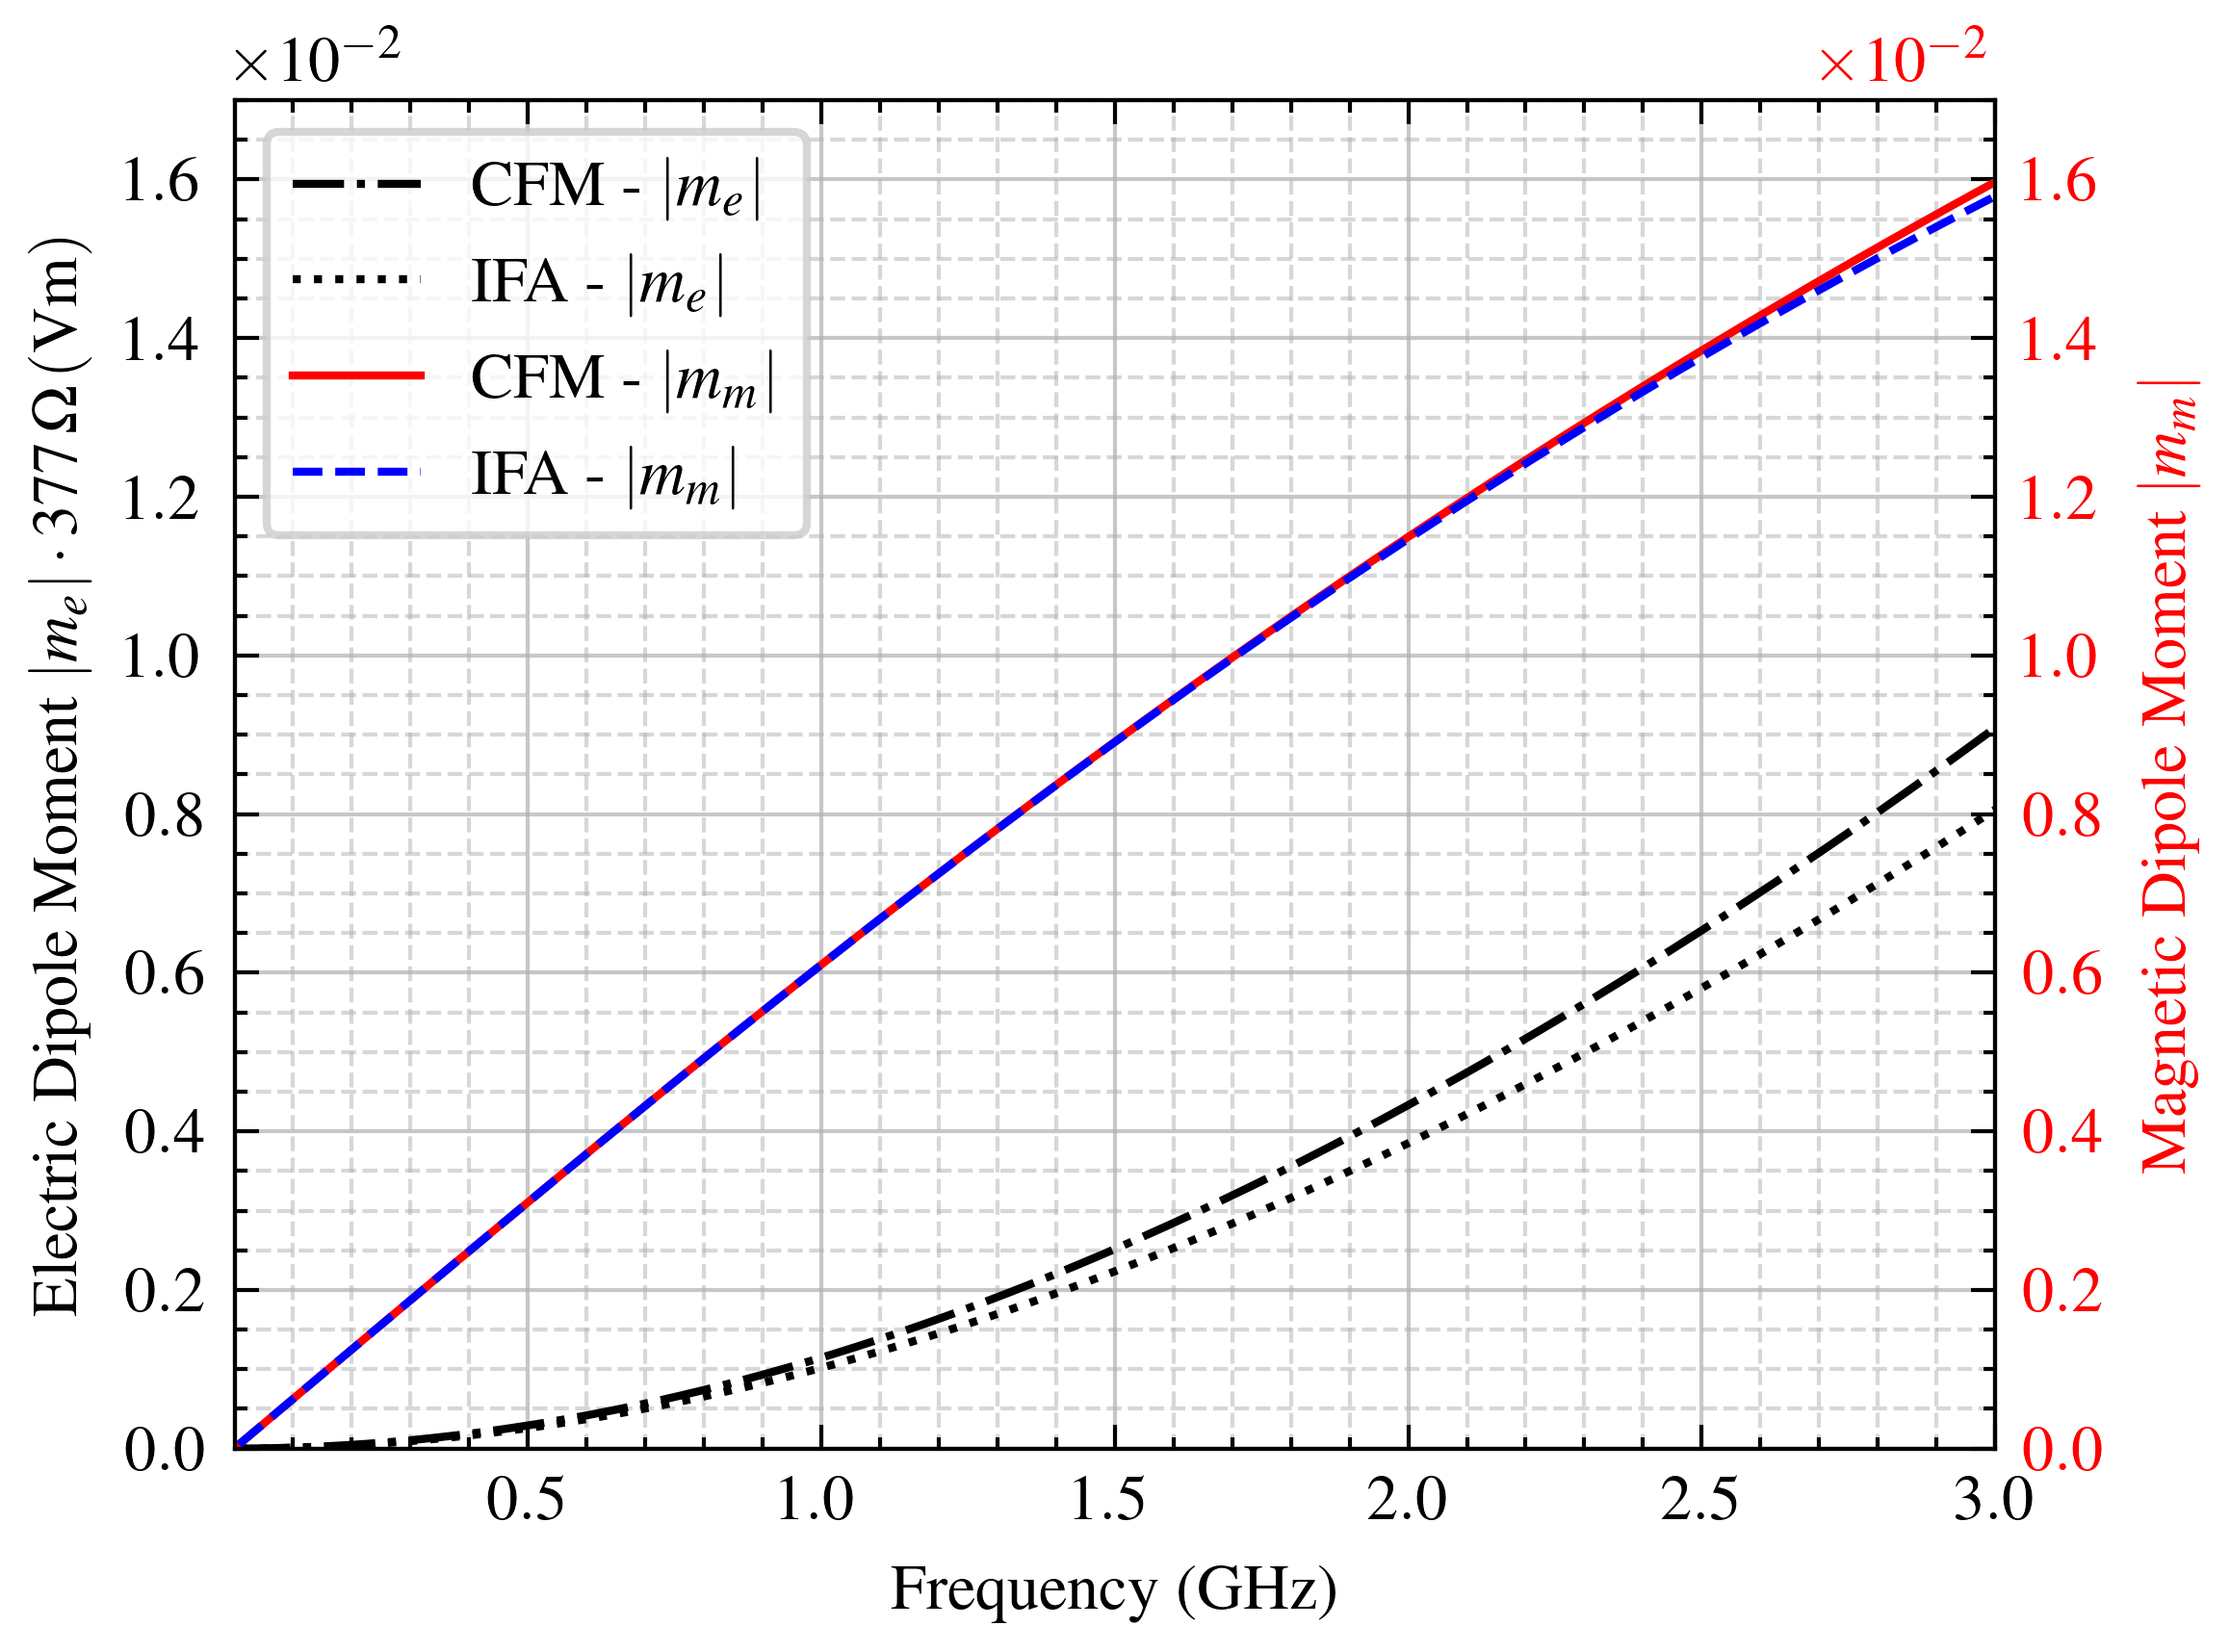
\includegraphics[width=1\linewidth]{content/img/cfm-ifa-moments}
		\caption{Equivalent dipole moments of IFA and CFM}
		\label{fig:cfm-ifa-moments}
	\end{subfigure}
	\caption{Geometries of IFA and CFM antenna, together with their equivalent dipole moments. The electric dipole moment $\mathbf{m}_e$ is weighted with the free space impedance $\eta_0$ to enable comparison with the magnetic dipole moment $\mathbf{m}_m$.}
	\label{fig:ifacfmmoments}
\end{figure}

The magnetic dipole moments $\mathbf{m}_m$ of the CFM and IFA, presented in \autoref{fig:cfm-ifa-moments}, are comparable to each other but smaller in magnitude than that of the loop antenna, despite sharing an identical loop area. This reduction is attributed to the additional linear arms of the CFM and IFA, on which charges accumulate. Through the continuity equation, this charge accumulation is coupled to the current distribution, redirecting current away from the loop and thereby reducing the conductive current. According to \eqref{eqn:e_a_closed_int} and \eqref{eqn:e_b_closed_int}, this reduction in conductive current directly weakens the magnetic coupling, resulting in a smaller $\mathbf{m}_m$.

Conversely, the electric dipole moment $\mathbf{m}_e$ of the CFM and IFA is significantly larger than that of the loop antenna. The additional linear arms introduce further charge accumulation, which enhances the displacement current coupling to the septum. According to \eqref{eqn:me_i}, this directly increases $\mathbf{m}_e$, as clearly reflected in the equivalent dipole moments shown in \autoref{fig:cfm-ifa-moments}.

In summary, the addition of a linear arm to the loop geometry reduces 
$\mathbf{m}_m$ while simultaneously enhancing $\mathbf{m}_e$, demonstrating 
that geometrical modifications of an inductive reference antenna modify electric and magnetic coupling without altering the fundamentally inductive character of the antenna.

\FloatBarrier